\chapter{Energy Landscape Methods}
\label{ch:methods}
\graphicspath{{methods/fig/}}

In this chapter we will explore some of the existing methods for energy landscape exploration.
Then we will discuss the advantages and disadvantages for each of the methods, including their use for elastic structures and other continuous systems.
It is not feasible to discuss all such methods, so we will restrict our focus to some of the most commonly used approaches.

Firstly, we will look at energy minimisation methods, which are central to the exploration of energy landscapes.
They are used to locate local minima in the landscapes, and are utilised in almost all energy landscape methods to find saddle points and minimum energy pathways.
So, efficient minimisation algorithms are crucial.

After this we will look at methods for locating transition states (TS).
These can use a single state to find a nearby TS, so-called single-ended methods, or can use two states that converge towards a TS from either side, known as double-ended methods.
Finally, we will look at some methods for locating minimum energy pathways using a chain of states.
These methods are also often referred to as double-ended transition state methods, while the bracketting methods are often overlooked.
However, here we will not be refer to them as such, and disambiguate between the two groups according to whether a method is primarily locating the pathway or the TS.



\section{Energy minimisation}

\subsection{Gradient descent}
Perhaps the simplest minimisation algorithm is gradient descent.
In this method a point on the landscape is iteratively refined by taking steps in the direction opposite to the gradient.
This causes the point to follow the path of steepest descent towards the local minimum.
Explicitly, the coordinates $\bm{x}_i$ at iteration $i$ are updated according to,
\begin{equation}
  \bm{x}_{i+1} = \bm{x}_i - \alpha_i \grad E(\bm{x_i}).
  \label{eq:lm-graddescent}
\end{equation}
The step size, $\alpha_i$, may be set to a single value, however this would slow down convergence, and may cause the method to diverge if it is too large.
A more common method is to use a line search (described below) to perform a one-dimensional optimisation in the direction of the step.

\subsubsection{Line search}
Given a search direction $\bm{p}$ (for gradient descent $\bm{p} =-\grad E(\bm{x})$) the aim of the line search is to find the step size, $\alpha$, that minimises the function $E(\bm{x}+\alpha\bm{p})$.
An exact solution could be found, but this is likely inefficient.
Instead, it is best to find a value that is good enough and then proceed with the next iteration of the method.
Two common ways of determining this are using the Wolfe conditions \cite{Wolfe1969,Wolfe1971} or a backtracking line search \cite{Armijo1966}.

The Wolfe conditions are that the objective function must reduce sufficiently (the Armijo rule), and that the gradient must also reduce sufficiently (the curvature rule):
\begin{gather}
  E(\bm{x}+\alpha\bm{p}) \le E(\bm{x}) + c_1 \alpha \bm{p} \cdot \grad E(\bm{x}),     \qquad \text{(Armijo rule)}
  \label{eq:lm-ls-armijo}
  \\
  - \bm{p} \cdot \grad E(\bm{x}+\alpha\bm{p}) \le - c_2 \bm{p} \cdot \grad E(\bm{x}). \qquad \text{(Curvature rule)}
  \label{eq:lm-ls-curvature}
\end{gather}
The parameters $c_1$ and $c_2$ must be chosen to satisfy $0 < c_1 < c_2 < 1$.
Each of these rules places a bound on the step size, with the Armijo rule placing a maximum bound, and the curvature rule enacting a minimum bound.

The backtracking line search is a little different.
The Armijo rule is still used to ensure that the step size is not too large, however the curvature rule is not.
Instead, the method first begins with a large step size and incrementally reduces it until it satisfies the Armijo rule.


\subsection{Newton's method}
Newton's method is a second order minimisation method that uses the Hessian to provide a faster rate of convergence than first order methods such as gradient descent.
Each iteration of this method effectively uses the gradient and curvature to fit a paraboloid to the energy landscape surface, and then proceed to the critical point.
As a result, this method may also find maxima or saddle points instead of local minima.

To obtain the step, $\bm{s}_i$, to take from a position $\bm{x}_i$ at iteration $i$, we consider the second-order Taylor expansion,
\begin{equation}
  E(\bm{x}_i + \bm{s}_i) = E(\bm{x}_i) +  \bm{s}_i^\mathrm{T} \grad E(\bm{x}_i) + \frac{1}{2} \bm{s}_i^\mathrm{T} \mathrm{H}(\bm{x}_i) \bm{s}_i,
\end{equation}
where $\mathrm{H}$ is Hessian matrix.
The step should take it to the critical point, where the gradient is zero,
\begin{equation}
  \grad E(\bm{x}_i + \bm{s}_i) = \grad E(\bm{x}_i) + \mathrm{H}(\bm{x}_i) \bm{s}_i = 0.
\end{equation}
So the step that should be taken at each iteration is
\begin{equation}
  \bm{s}_i = - \mathrm{H}^{-1}(\bm{x}_i) \  \grad E(\bm{x}_i).
  \label{eq:lm-newtonstep}
\end{equation}
Once the step has been found it is also possible to perform a line search along that direction.
This can be used to ensure that the energy always reduces and a minimum is found rather than a saddle point or maximum.


\subsection{L-BFGS}
The limited-memory Broyden-Fletcher-Goldfarb-Shanno (L-BFGS) algorithm \cite{Nocedal1980,Liu1989} addresses two difficulties associated with Newton's method.
The first is the calculation of the Hessian, which may be complicated or not known for many systems.
Furthermore, for an $n$-dimensional system it has a computational complexity of $O(n^2)$, so it can be computationally costly for many energy landscapes which have a very large number of dimensions.
The second is the inversion of the Hessian in \cref{eq:lm-newtonstep}, which is even more costly, scaling as $O(n^3)$.
Since L-BFGS is a quasi-Newtonian method which approximates \cref{eq:lm-newtonstep} rather than calculating the Hessian directly, it does not suffer from these same problems.

It is based upon the BFGS algorithm \cite{Fletcher1987}, which continually updates an approximation of the inverse Hessian matrix using the changes to the position and gradient at each iteration.
This prevents the need to know the Hessian, or perform the matrix inversion.
However, the whole matrix $\mathrm{H}^{-1}$ must still be calculated, with a complexity of $O(n^2)$.

L-BFGS addresses this by only storing several vectors representing changes in the positions and gradients of the past $m$ steps ($\bm{s}_j$ and $\bm{y}_j$ for $j=i-m,\ldots,i-1$, respectively), and the approximation of \cref{eq:lm-newtonstep} is calculated directly.
This bypasses the need to calculate the full inverse Hessian matrix, and results in a much lower complexity of $O(nm)$.
To do this, two sets of vectors ($q_j$ and $z_j$ for $j=i-m,\ldots,i$) are calculated iteratively based upon the recursive method used by BFGS.
The first vectors are given by
\begin{align}
  \bm{q}_i &= \grad E(\bm{x}_i),
  \label{eq:lm-lbfgs-q0}
  \\
  \bm{q}_j &= \bm{q}_{j+1} - \left( \frac{\bm{s}_j \cdot \bm{q}_{j+1}} {\bm{s}_j \cdot \bm{y}_j} \right) \bm{y}_j
    \quad \text{for} \quad j = i-1, \ldots, i-m.
  \label{eq:lm-lbfgs-q}
\end{align}
Then the second set of vectors are calculated as
\begin{align}
  \bm{z}_{i-m} &= - \left( \frac{\bm{s}_{i-1} \cdot \bm{y}_{i-1}} {\bm{y}_{i-1}^2} \right) \bm{q}_{i-m},
  \label{eq:lm-lbfgs-z0}
  \\
  \bm{z}_{j+1} &= \bm{z}_j - \left( \frac{\bm{s}_j \cdot \bm{q}_{j+1}} {\bm{s}_j \cdot \bm{y}_j} -
    \frac{\bm{z}_j \cdot \bm{y}_j} {\bm{s}_j \cdot \bm{y}_j} \right) \bm{s}_j
    \quad \text{for} \quad j = i-m, \ldots, i-1.
  \label{eq:lm-lbfgs-z}
\end{align}
The step to take is then given by $\bm{s}_i = \bm{z}_i$.
It is also generally desirable to carry out a line search in this direction to ensure that the step is acceptable and is going downhill.
This is then repeated until convergence is reached.


\subsection{FIRE}
Another useful method is the fast inertial relaxation engine (FIRE) \cite{Bitzek2006}.
Unlike the other methods this uses an inertial minimiser inspired by molecular dynamics.
This involves a velocity, $\bm{v}$, that quantifies the rate of change of the system coordinates, which is driven by the force $\bm{F} = - \grad E(\bm{x})$.
Additional modifications are also made to the velocity in order to drive it more quickly in the downhill direction, or stop if it is moving uphill,
\begin{equation}
  \bm{v} \rightarrow
  \begin{cases}
    \bm{v} + \alpha |\bm{v}| (\bm{\hat{F}} - \bm{\hat{v}}) & \text{if } \bm{v} \cdot \bm{F} > 0\\
    0 & \text{if } \bm{v} \cdot \bm{F} \le 0
  \end{cases}
  \label{eq:FireVelUpdate}
\end{equation}
where $\alpha$ parametrises the downhill velocity modification and $\Delta t$ is the timestep.
These values are also dynamically changed to accelerate the minimisation if it is successfully proceeding downhill:
If $\bm{v} \cdot \bm{F} > 0$ for the past five or more iterations, $\Delta t$ is increased by a factor of 1.1 until it reaches a defined maximum value, and $\alpha$ is reduced by a factor of 0.99.
Otherwise, if $\bm{v} \cdot \bm{F} \le 0$, $\alpha$ is reset to its starting value of 0.1, and the timestep is halved.
In summary the method follows the following algorithm:
\begin{enumerate}[leftmargin=*]
  \item Initialise coordinates $\bm{x}$, and velocity $\bm{v}=\bm{0}$.
  \item Calculate the force $\bm{F} = - \grad E(\bm{x})$.
  \item Update the velocity, $\bm{v} \rightarrow \bm{v} + \bm{F} \Delta t / m$.
  \item Modify the velocity according to \cref{eq:FireVelUpdate}.
  \item Update $\alpha$ and $\Delta t$ depending upon the value of $\bm{v} \cdot \bm{F}$.
  \item Update the position, $\bm{x} \rightarrow \bm{x} + \bm{v} \Delta t$.
  \item Check for convergence, otherwise return to 2.
\end{enumerate}


\subsection{Simulated Annealing}
For some applications, when the gradient is undefined or difficult to calculate it may be necessary to use a gradient-free minimisation algorithm.
This is most typically the case for discrete problems.
Simulated annealing \cite{Kirkpatrick1983} is one such algorithm that is based upon the thermodynamic annealing of metals.
This uses random displacements and chooses whether to accept them depending upon the change in energy.
Unlike the methods above, simulated annealing is primarily a global minimiser because it can jump into the basins of other minima and so is not simply restricted to finding the local minimum closest to its initial position.

For each iteration the random perturbation is chosen such that the new state is not too far from the previous.
This may be performed by adding small perturbations to each degree of freedom separately, or ensuring that the total displacement is below a certain value.
The probability of accepting this depends upon the energies of the proposed state, $E'$, and the current state, $E$, according to a Metropolis acceptance criteria \cite{Metropolis1953},
\begin{equation}
  P(E', E, T) =
  \begin{cases}
    1, & \text{if } E' \le E\\
    \exp( -(E'-E) / T ), & \text{if } E' > E
  \end{cases}
  \label{eq:lm-metropolis}
\end{equation}

The temperature, $T$, is reduced over the course of the simulation from a high initial temperature, $T_0$, to zero.
This allows the state to initially explore the entire configuration space, but it is steadily constrained to a single minimum.
Usually the rate of cooling should be sufficiently slow so that the state is remains at thermodynamic equilibrium, otherwise it is highly likely to get stuck in a local minimum rather than finding the global minimum.
This rate will depend upon the specific application, and it is hard to predict a reasonable value a priori.
The precise cooling schedule can use a variety of different functions, such as a linear reduction in temperature or an exponential decrease.

Simulated annealing may also be used to emulate local minimisation by setting $T=0$, ensuring that the energy can only decrease.
However, the method is not guaranteed to find the closest local minimum, because the random perturbations may still cause it to jump into the basin of another minimum.
The probability of this can be reduced by setting a small limit for the maximum perturbation, but it cannot be avoided entirely.


\subsection{Basin hopping}
Basin hopping is a related method for finding global minima \cite{Wales1997}.
Like simulated annealing, it employs Monte Carlo sampling and evaluates moves according to the criteria given in \cref{eq:lm-metropolis}.
However, there are two main differences between the methods.
Firstly and most significantly, the energy of each trial state is computed by performing a local minimisation.
This ensures that all states within a basin of attraction have the same energy for the acceptance test, effectively eliminating the barriers between adjacent basins.
The coordinates of the state may be left unchanged by the minimisation process, or they may be updated to the position of the local minimum.
The latter approach, given by Li and Scheraga \cite{Li1987}, is generally seen to be the more effective strategy \cite{Wales2004}.

The second notable difference is that the temperature is held constant throughout the simulation.
Instead of depending upon a changing temperature to adequately explore the energy landscape, the step size is adjusted dynamically to ensure that the average acceptance ratio aligns with a chosen value.

The basin hopping algorithm will tend towards deeper basins until it locates the global minimum.
However, the finite temperature also allows it to move to higher basins so that it can pass between multiple funnels in the landscape.
This allows it to successfully locate global minima, even in landscapes with multiple deep funnels.
To do this, the temperature must be approximately the size of the barriers separating funnels.
So if the funnels are particularly deep or the temperature is too low the method may potentially get stuck.


\subsection{Genetic algorithm}
Genetic algorithm is another method for performing global minimisation \cite{Katoch2021} that is based upon genetic evolution.
In contrast to the other methods that have been described, genetic algorithm does not optimise using a single state, but instead an ensemble of states.
Each iteration of the algorithm selects the fittest individuals (with the lowest energies) in the population which are used to produce a new generation.
These children are produced through a combination of crossover the parents genes, and mutation.

The selection of the parents generally occurs stochastically where the fitter individuals are more likely to be selected.
There are a number of such methods, but a simple approach that is often used is the roulette wheel selection.
For this, the probability that each individual is picked is proportional to their fitness (or inversely proportional to their energy),
\begin{equation}
  p(\bm{x}_i) = \frac{1}{E(\bm{x}_i)} \bigg/ \sum_j \frac{1}{E(\bm{x}_j)}.
\end{equation}
An approach known as elitism may also be used, where a small number of the most fit individuals are selected for the next generation without undergoing any changes.
This ensures that the best solutions are never lost and the global minimum estimate can only ever improve during the simulation.

For each child in the new generation the parents are randomly selected.
Typically, two parents are chosen, but more parents can be used.
Then, the most simple approach is to use uniform crossover, where each coordinate is randomly selected from each of the parents.
Alternatively, the parents' coordinates may be split at a random point and swapped, resulting in a block of coordinates from one parent and the remaining coordinates from the other.
This is known as one-point crossover, and can be generalised by splitting at a larger number of points.

The selection of the most fit individuals reduces the genetic diversity of the overall population and can lead to premature convergence, so mutation is used to keep the diversity high.
For discrete applications the genetic information of an individual can be expressed as a string of binary values.
Mutation is then performed by randomly flipping certain bits at a given probability, analogous to real genetic mutation.
However, for continuous systems mutation is usually carried out by altering each coordinate by a random amount chosen from a normal distribution.

For continuous applications it also can be helpful to consider hybrid methods \cite{El-Mihoub2006}.
These can be used to perform a gradient-based local minimisation on each individual when calculating the fitness.
This is also known as a Lamarckian genetic algorithm because of the ability for individuals to pass on what they have `learned'.
Performing the local search is beneficial because it can locate local minima much faster than using genetic algorithm alone.
Also, it may be useful for studying energy landscapes where the minima sit in deep wells, in which case the energy in the neighbouring region may be unrelated to the energy of the minima.

However, a local search may cause issues due to many duplicates, which can result in a lack of genetic diversity and stagnation of the population before reaching the global minimum.
One approach to resolve this is to remove individuals that are too close to another using a duplicate predation operator \cite{Manby1998,Cox2004}.
This ensures that the population remains diverse, so it can converge more quickly to the global solution, and also finds more local minima.
However, duplicate predation may result in too few parents if there are not many minima on the landscape, in which case more individuals would need to be initialised, or the method restarted.



\section{Single-ended transition state methods}\label{sec:lm-se}
One approach to locate saddle points is by evolving a single state such that it ascends up valleys in the landscape, effectively maximising one degree of freedom while minimising others.
Such methods are known as walker methods or single-ended transition state search methods.
We will discuss the climbing image, eigenvector-following, and dimer methods, although other methods also exist, such as the climbing string method \cite{Ren2013} or the Lanczos iterative method \cite{Malek2000}.

\begin{figure}[htb]
  \centering
  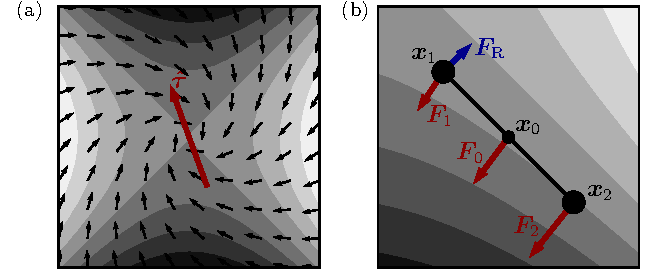
\includegraphics{single-ended.pdf}
  \caption{\label{fig:lm-singleended}
    (a) The effect of $\bm{\hat{\tau}}$ on the climbing image force in the vicinity of a saddle point (white is high energy, black is low).
        Here $\bm{\hat{\tau}}$ is pointing $20^\circ$ away from the optimal vertical direction, resulting in an inward spiralling force.
        The arrows show only the direction of the force.
    (b) The forces used to rotate a dimer, including the downhill forces on each state, $\bm{F}_i$, and the rotational force applied to state 1 about the midpoint, $\bm{F}_\mathrm{R}$.
  }
\end{figure}


\subsection{Climbing image}
The climbing image method \cite{Henkelman2000a,E2007} is perhaps the most simple single-ended method.
It involves minimising the energy of a state, but the gradient is inverted in a chosen direction, $\bm{\hat{\tau}}$, resulting in a driving force of the form,
\begin{equation}
  \bm{F} = - \grad E + 2 (\grad E \cdot \bm{\hat{\tau}}) \bm{\hat{\tau}}.
  \label{eq:lm-ci-force}
\end{equation}
An example of this force about a saddle point is shown in \cref{fig:lm-singleended}(a).

Because the gradient has been modified, this can no longer be considered a minimisation problem.
Therefore, optimisation methods that ensure that the energy decreases, such as line search, can not be used here.
This is also the case for most of the other energy landscape methods.

The climbing image is able to reach the TS so long as it starts sufficiently close to it and $\bm{\hat{\tau}}$ is approximately the direction of negative curvature at the TS.
If not, this method is likely to diverge.
Therefore, this method is often used in conjunction with other methods, especially pathway methods, in order to refine an initial estimate for the transition state, but it cannot usually locate a TS from a minimum.


\subsection{Eigenvector-following}
Unlike the climbing image method which requires the maximisation direction to be provided, the eigenvector-following method \cite{Cerjan1981,Munro1999} instead calculates it by finding the eigenvector with the lowest eigenvalue of the Hessian matrix, $\mathrm{H}$.
Also, because this direction is updated at each step, the state does not need to be initialised close to the TS.
The original method by Cerjan and Miller \cite{Cerjan1981} required calculating the inverse Hessian matrix, with later methods finding ways around the costly matrix inversion \cite{Wales1994}.
Munro and Wales then introduced the hybrid eigenvector-following method that did not require the Hessian matrix to be calculated at all, making it useful for large systems \cite{Munro1999}.

The method used by hybrid eigenvector-following to find the smallest eigenvalue is to first consider the following function for a vector $\bm{y}$,
\begin{equation}
  \lambda(\bm{y}) = \frac{\bm{y}^\mathrm{T} \mathrm{H} \bm{y}} {\bm{y}^2}.
\end{equation}
When this function is minimised with respect to $\bm{y}$ it will give the value of the smallest eigenvalue, $\lambda_\text{min}$, and $\bm{y}$ will be in the direction of the corresponding eigenvalue, $\bm{\hat{e}}_\text{min}$.
To do this without knowledge of the Hessian, $\lambda(\bm{y})$ is approximated using the function,
\begin{equation}
  \lambda(\bm{y}) \approx \frac{E(\bm{x}_0 + \delta\bm{y}) + E(\bm{x}_0 - \delta\bm{y}) - 2 E(\bm{x}_0)} {(\delta \bm{y})^2},
\end{equation}
where $\bm{x}_0$ is the position where we are evaluating the Hessian, and $\delta$ is a very small value.

Once the minimum eigenvalue and eigenvector have been found the state is stepped uphill along the eigenvector with a step size of
\begin{equation}
  h = \frac {2F} {\abs{\lambda_\text{min}} (1 + \sqrt{1 + 4 F^2 / \lambda_\text{min}^2})},
\end{equation}
with
\begin{equation}
  F = \grad E \cdot \bm{\hat{e}}_\text{min}.
\end{equation}
Then the energy is minimised along the hyperplane orthogonal to $\bm{\hat{e}}_\text{min}$.
This entire process is repeated, first finding the eigenvector then stepping uphill and minimising, until it converges to the saddle point.


\subsection{Dimer method}
The dimer method \cite{Henkelman1999,Heyden2005,Kastner2008} is a variant of the eigenvector-following method, that identifies the smallest eigenvector of the Hessian using a pair of close-lying states.
It does this by using the gradient on each state to generate a torque that turns the dimer to minimise the curvature.

By considering a close pair of states $\bm{x}_1$ and $\bm{x}_2$ with midpoint $\bm{x}_0$, each experiencing a force $\bm{F}_i = \grad E(\bm{x}_i)$ (as demonstrated in \cref{fig:lm-singleended}(b)), the rotational force applied to state 1 is found to be
\begin{equation}
\begin{aligned}
  \bm{F}_\mathrm{R} &= (\bm{F}_1 - \bm{F}_2) - [(\bm{F}_1 - \bm{F}_2) \cdot \bm{\hat{\tau}}] \bm{\hat{\tau}}\\
                    &= 2(\bm{F}_1 - \bm{F}_0) - 2[(\bm{F}_1 - \bm{F}_0) \cdot \bm{\hat{\tau}}] \bm{\hat{\tau}},
\end{aligned}
\end{equation}
where $\bm{\tau} = \bm{x}_1 - \bm{x}_0$.
This has been re-expressed using the force at the midpoint, because this is needed for the translation step, so one fewer gradient calculation is necessary.
This rotation force can be used to iteratively reorient the dimer until it reaches convergence.

Once this has occurred the dimer proceeds similarly to the climbing image method, maximising in the direction of the gradient while minimising in other directions using \cref{eq:lm-ci-force}.
However, if the dimer is located in a convex region where the curvature along the dimer is positive (such as close to minima) a different force is instead used to ensure that it does not get trapped:
\begin{equation}
  \bm{F} = (\grad E \cdot \bm{\hat{\tau}}) \bm{\hat{\tau}}.
\end{equation}



\section{Double-ended transition state methods}\label{sec:lm-de}
If both endpoints of a transition are known then single-ended methods are inadequate because they are not guaranteed to find the correct TS.
Instead, double-ended methods that converge towards the saddle from either side can be used.
Unlike pathway methods these do not typically require an initial estimate for the pathway, simplifying the process for applications with complex non-linear pathways.

There are a number of such methods, including the method introduced by Dewar, Healy, and Stewart (DHS) \cite{Dewar1984}, the step and slide method \cite{Miron2001}, the ridge-walking method \cite{Ionova1993}, and the double-ended surface walking method \cite{Zhang2013}.
Here we will focus on the first two.


\subsection{DHS method}
The DHS method \cite{Dewar1984} involves individually minimising each of the two states under a constant separation from the other state.
This separation is then steadily reduced until the method converges to the transition state.

Each iteration of the method involves first identifying which of the two states has the lowest energy.
This state is typically further from the transition state, so it is chosen to be minimised.
It is then brought towards the other, typically by about 5\%, and minimised under a fixed separation constraint.
After one or more iterations, this state gains a higher energy than the other and the minimisation switches to the other state.
The behaviour of this method is demonstrated in \cref{fig:lm-doubleended}.


\subsection{Step-and-slide method}
The step and slide method \cite{Miron2001} is similar to the DHS method, although, the roles are switched.
Instead of fixing the separation and minimising the energy, the separation is minimised at constant energy.
This is iteratively performed using a two-step process.
First, an energy is first chosen and the two states are `stepped' directly towards one another until they reach the isosurface for this energy.
Then, the states `slide' along this isosurface until the separation is minimised.
If the chosen energy is below that of the transition state then the two states will approach the TS.
Whereas, if it is too high, the states will meet and should be reverted back to their previous positions.
In this way, step and slide is able to provide an energy bound for the transition state.

In order to slide along the isosurface a bespoke minimisation procedure is required.
It must also be implemented in such a way that one state cannot accidentally jump over the saddle point, otherwise the method will fail.
For example, this may occur if the state is moved tangentially to the isosurface when close to the saddle.
Therefore, the approach used in ref.~\citenum{Miron2001} is to instead move one state downhill slightly according to the gradient and then step back up to the isosurface.
This is alternatively performed on each state until the separation has converged.

In order to choose the target energy for each iteration $E_\text{trial}$, the method uses maximum and minimum bounds for the transition state energy.
The minimum energy is given by the energies of the two states $E_{1,2}$, while the maximum energy, $E_\text{max}$, is updated any time the states combine after the slide.
Then the target energy can be chosen according to a binary search, $E_\text{trial} = (E_{1,2}+E_\text{max})/2$.
To initialise the method the maximum bound can be set by finding the maximum energy of a linear interpolation.
However, if the result is very large, it may be better to increase the energy by a set amount until an upper bound is found that way.

\begin{figure}[htb]
  \centering
  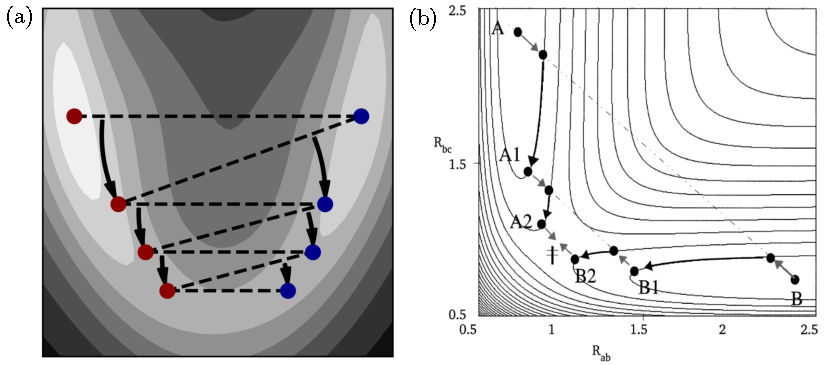
\includegraphics{double-ended.pdf}
  \caption{\label{fig:lm-doubleended}
    (a) A diagram demonstrating the behaviour of the DHS method.
    (b) An illustration of two iterations of the step and slide method.
        Adapted with permission from \cite{Miron2001}.
  }
\end{figure}



\section{Pathway methods}\label{sec:lm-pathway}
Once transition states have been identified, the full MEPs can be found by performing a downhill minimisation from either side of the saddle to the minima and tracking the trajectory.
To accurately follow the steepest descent, the step size of this minimisation should not be too large, and ideally a gradient descent method should be used.
However, other minimisation methods, such as L-BFGS, can give an approximation of the pathway, particularly for large and complex systems where gradient descent may be slow.

Alternatively, there are a number of commonly used methods that can directly find MEPs between two end points.
Each of these approaches utilise a chain of states $\lbrace \bm{x}_1, ..., \bm{x}_N \rbrace$, where each state contains a full set of system coordinates.
This chain can be initialised as a linear interpolation between the two end states, but for some systems more complex pathways may be required \cite{Ionova1993,Chu2003,Wales2012a}.
The energy of the chain is then minimised while keeping the states equally separated until it converges to the MEP.
Convergence is satisfied when the gradient orthogonal to the local pathway tangent vector goes to zero for every state in the chain,
\begin{equation}
  \grad^\perp E(\bm{x}_i) = \grad E(\bm{x}_i) - (\bm{\hat{\tau}} \cdot \grad E(\bm{x}_i)) \bm{\hat{\tau}},
\end{equation}
where $\bm{\hat{\tau}_i}$ is the tangent vector to the pathway at image $\bm{x}_i$ along the chain.

These methods are also often used in order to find the approximate locations of transition states, which occupy local maxima along the MEP.
While these methods generally do not precisely find these transition states, they can be used in conjunction with a single-ended TS search method for this purpose.

A number of pathway search methods have been proposed, although here we will focus on two commonly used approaches: the nudged elastic band (NEB) and string methods, as well as some of their variants.

\begin{figure}[htb]
  \centering
  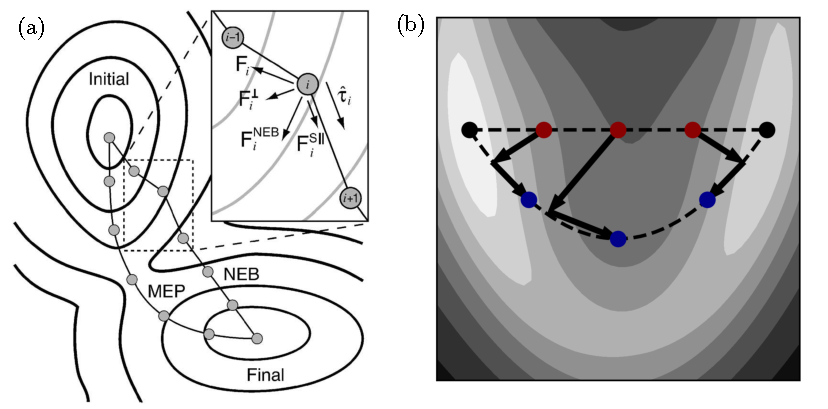
\includegraphics{pathway.pdf}
  \caption{\label{fig:lm-pathway}
    (a) A diagram showing how NEB converges to the MEP for a 2D landscape.
        The inset shows a schematic of the forces on an state in the chain.
        Adapted with permission from \cite{Sheppard2008}.
    (b) A schematic illustrating how the string method evolves.
        The arrows show the partial minimisation followed by a reparametrisation along the new interpolation.
  }
\end{figure}


\subsection{Nudged elastic band method}\label{sec:lm-neb}
The core feature of NEB methods \cite{Henkelman2000,Trygubenko2004} are that the states are kept separated along the chain using elastic spring interactions.
Therefore, the aim of the method can be considered to minimise the following total energy of the string,
\begin{equation}
  E_\text{NEB} = \sum_{i=1}^N \left[ E(\bm{x}_i) + \frac{1}{2} k \sum_{j=i+1}^N |\bm{x}_i - \bm{x}_j|^2 \right],
  \label{eq:lm-neb-energy}
\end{equation}
where $k$ is a parameter for the spring constant between the states.
However, a couple of modifications (`nudges') to the gradient of \cref{eq:lm-neb-energy} are made to reduce unwanted interference between the two contributions.
Firstly, the gradient of the underlying potential is projected perpendicular to the tangent vector, $\bm{\hat{\tau}}_i$.
This prevents the images from sliding down the pathway and ensures that the potential does not affect the parametrisation of the path, only its course.
The second modification aims to reduce the corner cutting around bends in the pathway by using only the component of the spring force parallel to the tangent vector.
Therefore the total gradient on state $i$ in the chain is
\begin{equation}
  \bm{G}_{\text{NEB},i} = \grad^\perp E(\bm{x}_i) + \bm{G}_{\text{S},i}^\parallel,
  \label{eq:lm-neb-gradient}
\end{equation}
where
\begin{gather}
  \bm{G}_{\text{S},i}^\parallel = (\bm{\hat{\tau}}_i \cdot \bm{G}_{\text{S},i}) \bm{\hat{\tau}}_i\\
  \bm{G}_{\text{S},i} = k (\bm{x}_{i+1} + \bm{x}_{i-1} - 2\bm{x}_i).
\end{gather}

The tangent vector at each point can be computed in a few ways.
The simplest approach is to use central difference between the points and normalise the result,
\begin{equation}
  \bm{\hat{\tau}_i} = \frac{\bm{x}_{i+1} - \bm{x}_{i-1}} {\abs{\bm{x}_{i+1} - \bm{x}_{i-1}}}.
\end{equation}
However, an approach that provides better results in areas of high curvature is to bisect the tangents given by forward and backward difference \cite{Henkelman2000},
\begin{equation}
  \bm{\tau}_i = \frac{\bm{x}_{i+1} - \bm{x}_{i}} {\abs{\bm{x}_{i+1} - \bm{x}_{i}}} +
                \frac{\bm{x}_{i} - \bm{x}_{i-1}} {\abs{\bm{x}_{i} - \bm{x}_{i-1}}}
  \quad\text{and}\quad
  \bm{\hat{\tau}}_i = \frac{\bm{\tau}_i}{\abs{\bm{\tau}_i}}.
  \label{eq:lm-neb-taubisect}
\end{equation}

A variant of NEB known as the doubly-nudged elastic band method (DNEB) brings further improvements to the method \cite{Trygubenko2004}, and has since seen widespread use.
This improves stability by introducing an additional term to the NEB gradient, \cref{eq:lm-neb-gradient}, such that the perpendicular component of the spring force is not completely removed.
This correction term is
\begin{equation}
  \bm{G}_\text{S}^* = \bm{G}_\text{S}^\perp - (\bm{G}_\text{S}^\perp \cdot \grad^\perp E) \grad^\perp E.
\end{equation}

The states along the chain in NEB and DNEB are unlikely to provide a particularly accurate approximation to the transition state, especially if there is significant corner cutting due to the spring interaction.
Therefore they are often used in hybrid methods with single-ended transition search methods, such as climbing image \cite{Henkelman2000a}, or eigenvector-following \cite{Trygubenko2004}.
Once the chain has converged these can be run from the highest energy state, or, can be applied to the highest state at the same time as the elastic band is minimised.
The latter requires some extra care because it is possible for the climbing state to diverge if it starts too far from the transition state.


\subsection{String method}\label{sec:lm-string}
The string method \cite{E2002,E2007} shares many similarities with NEB, however it differs essentially by the process that keeps the states separated along the chain.
Instead of using a spring force, the states are reparameterised along the pathway occasionally throughout the minimisation.

In the originally proposed method \cite{E2002} the states in the chain are driven downhill according to the gradient of the potential orthogonal to the direction of the chain.
Explicitly, for state $i$ along the chain this driving force would be,
\begin{equation}
  \bm{F}_i = - \grad E_i + (\bm{\hat{\tau}}_i \cdot \grad E_i) \bm{\hat{\tau}}_i.
\end{equation}
In a later modification to the method \cite{E2007} this driving force was simplified to remove the orthogonal projection because the reparametrisation step makes this unnecessary, leaving $\bm{F}_i = - \grad E_i$.
The tangent vector can be simply computed according to the difference between the neighbouring states, $\bm{\hat{\tau}}_i = (\bm{x}_{i+1} + \bm{x}_{i-1}) / |\bm{x}_{i+1} + \bm{x}_{i-1}|$.

After a certain number of minimisation iterations have passed the states must be reparametrised along the chain.
A suitable choice for this depends upon the system and the minimisation algorithm.
This reparametrisation may be performed using either a linear, or a cubic-spline interpolation along the set of points.
Then the new points can be equally separated along the interpolation.
The number of these new points does not necessarily need to be same as the previous step, which can make it easy to refine the pathway over time.
Additionally, the points do not need to be evenly distributed, and could instead be clustered close to the transition state by weighting the length of the interpolated path according to the local value of the potential \cite{E2007}.

Similar to NEB it is possible to use a hybrid method with climbing image \cite{E2007} or eigenvector-following in order to accurately find the transition state.
In this case, the state with the highest energy using the chosen method and should be left out of the reparametrisation step.
Another climbing image / string method hybrid, called the climbing string method, has also been proposed \cite{Ren2013}.
However, unlike the other methods, this is a single-ended saddle point search method.
This uses the string of states to guarantee that it has not left the basin of attraction for a minimum rather than for locating a MEP.


\section{Methods comparison}
\subsubsection{Minimisation}
\begin{table}
  \begin{tabularx}{\textwidth}{lCCCCC}
    \hline\hline
    Method              & Local  & Global & Gradient & Hessian & Ensemble\\
    \hline
    Gradient descent    & \cmark & \xmark & \cmark   & \xmark  & \xmark\\
    L-BFGS              & \cmark & \xmark & \cmark   & \xmark  & \xmark\\
    FIRE                & \cmark & \xmark & \cmark   & \xmark  & \xmark\\
    Newton's method     & \cmark & \xmark & \cmark   & \cmark  & \xmark\\
    Simulated annealing & \cmark & \cmark & \xmark   & \xmark  & \xmark\\
    Basin hopping       & \xmark & \cmark & \cmark   & \xmark  & \xmark\\
    Genetic algorithm   & \xmark & \cmark & \xmark   & \xmark  & \cmark\\
    \hline\hline
  \end{tabularx}
  \caption{
    A comparison of the different minimisation methods, indicating which can be used as local or global minimisers, which require the gradient or the Hessian, and which use an ensemble of states.
  }
\end{table}
Minimisation methods that use the Hessian, like Newton's method, generally provide faster convergence compared to other methods.
However, the calculation of the Hessian can become the limiting factor if the number of degrees of freedom is large, which it generally is in the continuous systems that we are interested in.
Since L-BFGS is quasi-Newtonian, it benefits from this faster convergence without being bogged down by the calculation of the Hessian, therefore it is ideal for our purpose.

FIRE is also a good option with convergence speeds approaching that of L-BFGS \cite{Bitzek2006}, so it is a good alternative for cases where L-BFGS has difficulty.
It is also more amenable to parallelisation along the degrees of freedom, because there are much fewer vector magnitudes and dot products calculated per iteration compared to L-BFGS.
On the other hand, FIRE has a free parameter, the maximum time step, which can require some tuning for each system and makes the method a little more difficult to use.

As for simulated annealing, it is primarily a global minimiser, but it can also be used to find local minima.
Compared to L-BFGS and FIRE it converges much more slowly, and the random perturbations make it possible to jump into the basin of another minima.
Therefore, where possible other methods should be used, but it is particularly useful if the gradient cannot be calculated or is undefined.

However, when it comes to global optimisation or locating multiple minima, basin hopping and the genetic algorithm tend to win out.
For genetic algorithm, the ensemble of states provides a much larger accessible search region, resulting in better performance for most problems \cite{Sexton1999,Kerr2019}.
Furthermore, it is well suited to parallelisation because each state can be run separately, with a minimal number of interactions in each generation.
As for basin hopping, it is particularly attractive because of its simplicity, the only variable parameter being the temperature.
This makes it more straightforward to apply to new systems in comparison to simulated annealing or genetic algorithm, which depend heavily upon the choice of cooling schedule and genetic operators, respectively, as well as their related parameters.

\subsubsection{Transition states and pathways}
\begin{table}
  \begin{tabularx}{\textwidth}{lCCCCC}
    \hline\hline
    Method          & Number of states & TS from endpoints & Can find multiple TS & No interpolation\\
    \hline
    Single-ended TS & 1                & \xmark            & \xmark               & \cmark \\
    Double-ended TS & 2                & \cmark            & \xmark               & \cmark \\
    Chain-of-states & $\ge 3$          & \cmark*           & \cmark*              & \xmark \\
    \hline\hline
  \end{tabularx}
  \caption{
    A comparison of the three types of TS and pathway methods, including the number of states that are optimised, if the method can find one or multiple TS between two chosen endpoints, and if an interpolation is required.
    An asterisk indicates a hybrid method is required.
  }
\end{table}
Single-ended search methods are generally efficient at locating saddle points quickly.
This makes them particularly well suited for surveying large numbers of transition states or refining estimates, such as those obtained from chain-of-states methods.
However, if a specific pathway between two known end states is of interest, single-ended methods are often inadequate and double-ended methods and chain-of-states methods should be used instead.

The simplicity of the climbing image method makes it excellent for refining transition state estimates, but it cannot usually be started far from the transition state, such as from minima.
The requirement for a tangent vector estimate also restricts its use.
The eigenvector-following and dimer methods solve these issues and can be used in most situations, but their success depends strongly upon the number of iterations allowed when calculating the uphill direction and the corresponding convergence criteria.
This can also take some time to adequately converge for large numbers of degrees of freedom.
If there are zero eigenmodes of the Hessian, such as global translation and rotation, then the dimer and eigenvector-following methods can also struggle and special consideration is required.

For finding the transition states and pathways between two end points, the choice between using double-ended transition state methods or chain-of-state methods will depend upon the situation.
Chain-of-states methods will be preferable if full pathways are desired, or precise transition states are not required.
Likewise, if there are many intermediate minima and transition states, which is often the case for particulate systems, chain-of-states methods can identify the approximate locations for many of these at once.
Chain-of-states methods are also more reliable, whereas double-ended methods can often fail to locate a transition state.
As a result, chain-of-states methods are much more widely used than other methods.
However, double-ended bracketting methods can be particularly efficient for finding transition states for pathways with no (or very few) intermediate minima.
This is especially true if the pathways are highly non-linear on the landscape, where chain-of-states methods require a large number of images to accurately approximate the pathway.
It can also make it difficult to choose an appropriate initial pathway estimate, which is necessary for chain-of-states methods.
These advantages make double-ended methods attractive for elastic structures and other continuous systems, which have comparatively few minima, yet complex, non-linear pathways.

Comparing the double-ended TS methods, we find that each has different advantages and disadvantages.
The DHS method is particularly simple to implement and use, and it can be good for obtaining the TS within a certain distance error.
However, because only one state is minimised at a time, the distance must be reduced quite slowly for it not to pass over the ridge.
As for the step and slide method, it is useful for getting a bound on the energy of the transition state.
However, the minimisation along a constant energy surface requires a more complicated implementation that is not as efficient as standard minimisation algorithms.
Also, it can be hard to know how much to initially increment the energy, if it is too large or too small the method may take a lot longer to converge.

Of the pathway methods, both DNEB and string methods have a comparable effectiveness.
Each can be advantageous for different systems and sets of parameters, but it is difficult to know which will be better a priori \cite{Koslover2007}.
